% ROHC conference for Capitole du Libre 2018
%
% The conference is about the ROHC library (https://rohc-lib.org/). It was
% given at  Capitole du Libre 2018 (https://2018.capitoledulibre.org/).
%
% The slides (except the projet and company logos) are Published under the
% CC BY-NC-SA 4.0 license (https://creativecommons.org/licenses/by-nc-sa/4.0/).
%
% Author: Didier Barvaux <didier@rohc-lib.org>

\documentclass[utf8]{beamer}
\mode<presentation>
\title{ROHC: compression of \\IP, UDP, RTP, TCP headers}
\author[Viveris]{Didier Barvaux, Viveris \\ {\tiny didier.barvaux@toulouse.viveris.com} \\ {\tiny didier@rohc-lib.org} \\ {\tiny slides published under CC BY-NC-SA 4.0}}
\date[Formation]{Capitole du Libre, Toulouse, 2018}

\usetheme{Warsaw}
\usecolortheme{whale}

\usepackage{listings}
\lstdefinestyle{mystyle}{
    basicstyle=\scriptsize
}
\lstset{style=mystyle}

\begin{document}

% Title
\begin{frame}
		\titlepage
\end{frame}

% Agenda
\begin{frame}
	\frametitle{Agenda}
	\tableofcontents[hideallsubsections]
\end{frame}

% Myself
\begin{frame}
	\frametitle{Me}
	\begin{block}{}
		\begin{columns}
			\begin{column}[T]{75mm}
				\begin{itemize}
					\item 2005: ENSEEIHT diploma
					\item 2005: daily job at Viveris {\tiny https://www.viveris.fr/}
					\item 2007: start working on ROHC library {\tiny https://rohc-lib.org/}
					\item ...
					\item 2018: still working at Viveris ;-)
					\item 2018: still working on ROHC library ;-)
				\end{itemize}
			\end{column}
			\begin{column}[T]{25mm}
				\begin{figure}
					
\includegraphics[height=15mm]{images/viveris_logo.png}
				\end{figure}
				\begin{figure}
					
\includegraphics[height=13mm]{images/rohc_logo.png}
				\end{figure}
			\end{column}
		\end{columns}
	\end{block}
\end{frame}


%%%%%%%%%%%%%%%%%%%%%%%%%%%%%%%%%%%%%%%%%%%%%%%%%%%%%%%%%%%%%%%%%%%%%%%%%%%%%


\section{Header compression}

\subsection{problem statement}
\begin{frame}
	\frametitle{Header compression: why?}
	\begin{block}{Header size is a concern on network links}
		\pause
		\begin{itemize}
			\item Voice Over IP (VoIP): 40B headers + 20B payload = 60B
			\item TCP Acknowlegments: 52B headers + 0B payload = 52B
		\end{itemize}
	\end{block}
	\pause
	\begin{block}{Compressed packets}
		\begin{itemize}
			\item Voice Over IP (VoIP): 1B header + 20B payload (65\% saved)
			\item TCP Acknowlegments: 4 bytes (92\% saved)
		\end{itemize}
	\end{block}
\end{frame}
\begin{frame}
	\frametitle{Is header compression still useful?}
	\pause
	\begin{block}{An old idea...}
		\begin{itemize}
			\item designed for low-speed serial links in 1990
			\item today network links are much larger
		\end{itemize}
	\end{block}
	\pause
	\begin{block}{...but still useful}
		\begin{itemize}
			\item slow links still exists (satellite, mobile...)
			\item larger links are congested
			\item data traffic may be expensive on links (satellite, mobile)
		\end{itemize}
	\end{block}
\end{frame}


%%%%%%%%%%%%%%%%%%%%%%%%%%%%%%%%%%%%%%%%%%%%%%%%%%%%%%%%%%%%%%%%%%%%%%%%%%%%%


\section{The ROHC protocol}

\subsection{definition}
\begin{frame}
	\frametitle{What ROHC is?}
	\begin{block}{RObust Header Compression (ROHC)}
		A network protocol that compresses away protocol headers
	\end{block}
	\pause
	\begin{block}{Objectives}
		\begin{itemize}
			\item lossless
			\item efficient
			\item robust to packet loss
			\item extensible framework {\tiny IPv4, IPv6, UDP, UDP-Lite, RTP, TCP, ESP, GRE...}
		\end{itemize}
	\end{block}
	\pause
	\begin{block}{IETF standard \tiny{https://www.ietf.org/}}
		\begin{itemize}
			\item \small{ROHCv1 (2001)}
			\item \small{ROHCv2 (2008)}
			\item \small{ROHC-TCP (2013)}
		\end{itemize}
	\end{block}
\end{frame}

\subsection{protocol}
\begin{frame}
	\frametitle{Main principles: only headers are compressed}
	\includegraphics[height=65mm]{images/rohc_only_headers_all.png}
\end{frame}

\begin{frame}
	\frametitle{Main principles: information redundancy}
	\begin{block}{redundancy inside one single network packet}
		avoid transmitting well-known or inferred fields
		\includegraphics[width=110mm]{images/rohc_redundancy_one_packet.png}
	\end{block}
\end{frame}

\begin{frame}
	\frametitle{Main principles: information redundancy}
	\begin{block}{redundancy between several network packets of one stream}
		transmit static fields a few times
		\includegraphics[width=110mm]{images/rohc_redundancy_one_flow.png}
	\end{block}
\end{frame}

\begin{frame}
	\frametitle{Main principles: packet classification}
	\begin{block}{classify packets by streams to optimize redundancy}
		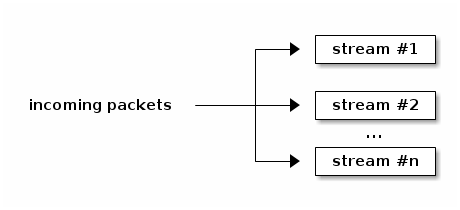
\includegraphics[height=60mm]{images/rohc_classification.png}
	\end{block}
\end{frame}

\begin{frame}
	\frametitle{Main principles: LSB encoding}
	\begin{block}{Least Significant Bits encoding}
		\begin{itemize}
			\item designed to compress small changes
			\item examples: RTP sequence number, TCP sequence number
		\end{itemize}
		\includegraphics[width=110mm]{images/rohc_lsb.png}
	\end{block}
\end{frame}

\begin{frame}
	\frametitle{Main principles: W-LSB encoding}
	\begin{block}{Window-based Least Significant Bits encoding}
		\begin{itemize}
			\item designed to compress small changes {\bf in a robust way}
			\item examples: RTP sequence number, TCP sequence number
		\end{itemize}
		\includegraphics[width=110mm]{images/rohc_wlsb.png}
	\end{block}
\end{frame}



%%%%%%%%%%%%%%%%%%%%%%%%%%%%%%%%%%%%%%%%%%%%%%%%%%%%%%%%%%%%%%%%%%%%%%%%%%%%%


\section{The ROHC library}

\subsection{history}
\begin{frame}
	\frametitle{History}
	\begin{block}{}
		\begin{itemize}
			\item 2003: initial version by Lulea University of Technologies
			\item 2007: internal fork by TAS, CNES, and Viveris Technologies
			\item 2009: public version of the fork (GPLv2+)
				\pause
			\item 2012: ROHCv1 IP/ESP profile
			\item 2013: beta IP/TCP profile + Linux kernel
			\item 2014: LGPLv2 license
				\pause
			\item 2016: IP/TCP profile
			\item 2017: Context Replication for IP/TCP profile
			\item 2018: ROHCv2 IP-only, IP/ESP and IP/UDP profiles
		\end{itemize}
	\end{block}
\end{frame}

\subsection{usage}
\begin{frame}[fragile]
	\frametitle{Usage example}
	\begin{block}{Compressing one IP/UDP/RTP packet}
	\begin{lstlisting}[language=C]
struct rohc_comp *compressor;
...
compressor =
	rohc_comp_new2(ROHC_SMALL_CID, ROHC_SMALL_CID_MAX,
	               gen_random_num, NULL);
rohc_comp_enable_profile(compressor, ROHC_PROFILE_RTP);
...
rohc_compress4(compressor, ip_packet, &rohc_packet);
...
rohc_comp_free(compressor);
	\end{lstlisting}
	\end{block}
	\scriptsize{API documentation, tutorials and examples on https://rohc-lib.org/support/documentation/}
\end{frame}

\subsection{compression efficiency}
\begin{frame}
	\frametitle{Compression efficiency}
	30-minute VoIP call\\
	{\tiny 90000 60-byte IPv4/UDP/RTP packets every 20 ms}
	\begin{figure}
		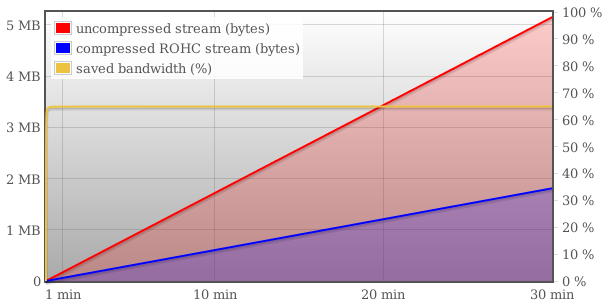
\includegraphics[height=50mm]{images/rohc_perfs.png}
	\end{figure}
\end{frame}

\subsection{recent changes}
\begin{frame}
	\frametitle{Recent changes}
	\begin{block}{Latest version 2.2.0 released on April 2018}
		\begin{itemize}
			\item add ROHCv2 IP-only, IP/ESP and IP/UDP profiles
			\item improve interoperability on ROHCv1 standards
			\item Wireshark dissector in Lua
		\end{itemize}
	\end{block}
	\pause
	\begin{block}{Next version 2.3.0 to be released}
		\begin{itemize}
			\item partial ROHCv2 IP/UDP/RTP profile
			\item improve interoperability on ROHCv1 standards
			\item improve robustness on lossy mediums
			\item better CPU and memory performances
		\end{itemize}
	\end{block}
\end{frame}

\begin{frame}
	\frametitle{A way to improve skills}
	\begin{block}{Skills I learned with the project}
		\scriptsize
		\begin{itemize}
			\item C language and compilers {\tiny + Python module, Lua, shell...}
			\item dev tools {\tiny autotools, Bzr, Git, vim}
			\item continuous integration {\tiny Travis CI, Buildbot}
			\item static analysis {\tiny clang, cppcheck, coverity}
			\item unit tests {\tiny 88\% LOC coverage computed by gcov/lcov}
			\item runtime analysis {\tiny valgrind, asan/ubsan, AFL fuzzer}
			\item debug tools {\tiny gdb, strace, perf, tcpdump, wireshark, tshark}
			\item software hardening {\tiny capabilities, seccomp-bpf, namespaces}
			\item documentation {\tiny Doxygen, man pages}
			\item packaging {\tiny ebuild, RPM, DEB}
		\end{itemize}
	\end{block}
	\begin{block}{Skills I would like to learn in the future}
		\scriptsize
		\begin{itemize}
			\item Rust
			\item Meson
		\end{itemize}
	\end{block}
\end{frame}


%%%%%%%%%%%%%%%%%%%%%%%%%%%%%%%%%%%%%%%%%%%%%%%%%%%%%%%%%%%%%%%%%%%%%%%%%%%%%

\end{document}

